\section{Homotopy}
\label{sec:homotopy}

Homotopy classes of curves are important  because...
In this section, we share applications
where the Gauss-Bonnet theorem is used to determine
if curve on a surface is contractible and find
the shortest path homotopic to a given path..


\subsection{Homotopy Testing on Surfaces}

In a video lecture Erickson describes an algorithm
to determine if a curve on a surface is contractible \cite{erickson-lecture}.
The algorithm relies on the Gauss-Bonnet theorem.

Here a we have a combinatorial surface that we call a map denoted $\Sigma.$
A curve is a walk, or alternating sequence of vertices
and edges, in the $\Sigma$.
A \EMPH{homotopy} between two closed curves $\gamma_1$ and $\gamma_2$ that 
share a point $p_0$ is a continuous map $H\colon [0,1]\times \Sp^1 \to \mathbb{R}^2$ 
such that $H(0,\cdot)=\gamma_1$, $H(1,\cdot)=\gamma_2$, and $H(s,0)=p_0=H(s,1)$.

On a combinatorial surface, homotopies can be decomposed
into discrete moves called edge spikes, edge unspikes  and face flips.

The question we consider is: Given a closed walk $W$ in a map $\Sigma$ is there a finite
sequence of moves that reduces the curve to a trivial walk?

\begin{figure}[htb]
\centering
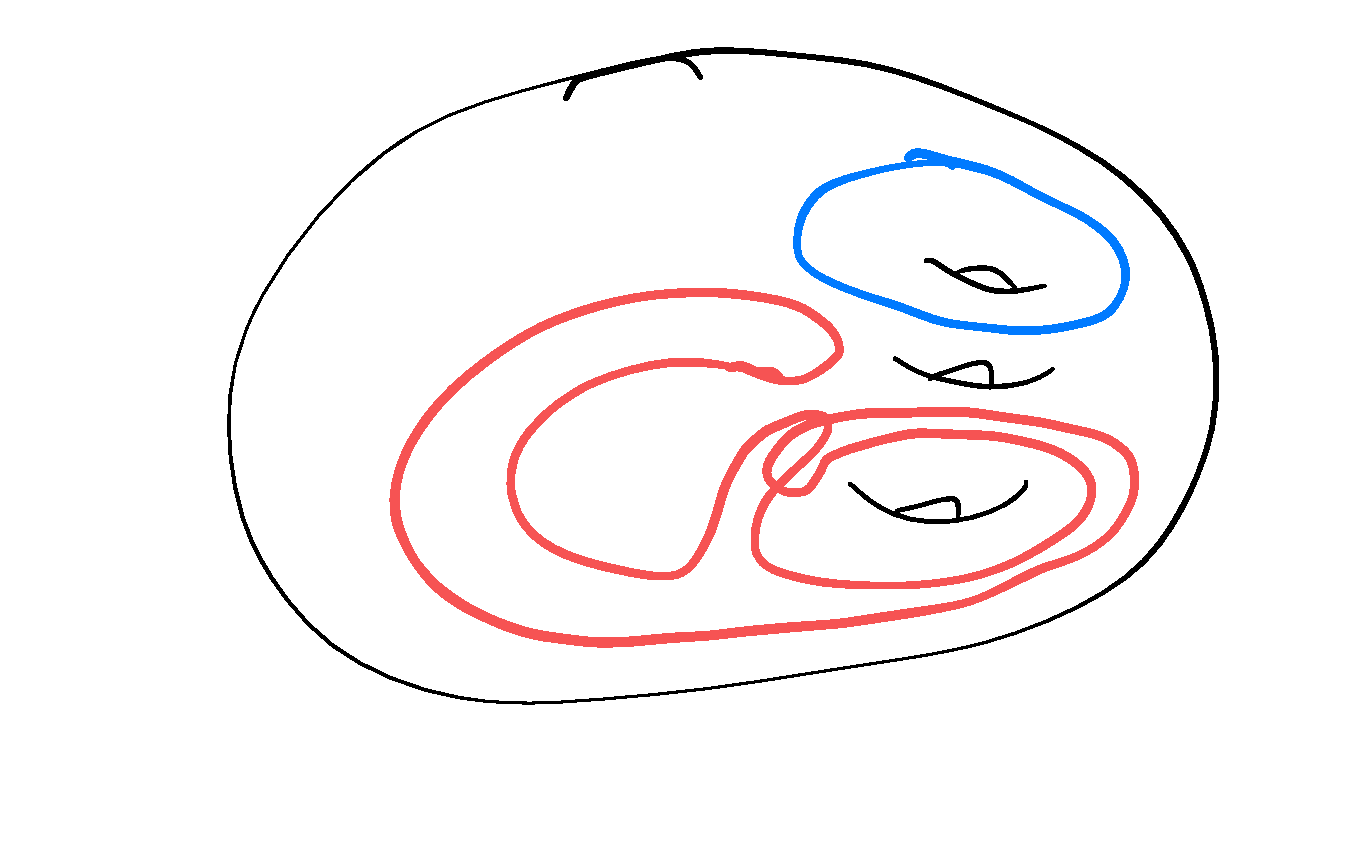
\includegraphics[width=.3\textwidth]{homotopy/contractable}
\caption{The blue curve is not contractable, the red curve is contractable.}
\label{fig:contractable}
\end{figure}

Transform $\Sigma$ into a system of loops.  
Take tree co-tree decomposition $(T,L,C)$
contract $T$, delete $C$ get system of loops $\Delta$.
If we contract an edge in $W$, delete the edge from $W$.
If we delete and edge $e\in W$, face flip to avoid the deleted edge.
Get a new walk $\hat{W} \in \Delta$ homotopic to $W\in \Sigma$
now only have one vertex. Then, $\hat{W}$ has one vertex
with degree $4g$, one face with $4g$ edges, and $2g$ loops.

The length of the walk increases by at most $2g$.

Slice along all loops to lift to the universal cover, where we glue
together infinite copies of the $4g$-gon. Get hyperbolic geometry
in the Poincare disk model. 

Big idea: a curve is contractible closed walk in $\Sigma$
if and only if the walk is closed in the universal covering space.
Thus, our problem is equivalent to the following: Given a walk
in the universal cover of a system of loops, is it closed?
All vertices look the same, how do you know if you ended where
you started?

Look for spurs or taking and instances where we talk the long way around a face, 
shorten the walk.
Any nontrivial contractible cycle contains either a spur or a bracket \cite{gertsen-short-1990}.
\begin{lemma}[Dehn's Lemma]\label{lem:dehn}
If $g\geq 2,$ then any nontirival closed walk has either a spur
or $4g-2$ consecutive edges on the boundary of a face.
\end{lemma}
\begin{proof}
Sketch: Gauss-Bonnet Theorem.
Define curvature $k(f)=1-\sum \alpha{a}$,
$k(v)=1-\frac{1}{2}\deg(v)+\sum_{v\in V} \alpha(\epsilon)$.
Since we are on the disk, by the Gauss-Bonnet theorem
$$\sum_v k(v)+\sum_f k(f) =1.$$

Each face has $4g$ edges, each internal  vertex has degree $4g$
and each  boundary vertex  has degree less than $4g$.
The angle of each angle on a face  is $\frac{1}{4}$,
thus, $k(f)=1-g<0,$ for internal vertices  $k(v)=1-g<0$ and for all
vertices on the boundary, $k(v)=\frac{3}{4}-\frac{\deg(v)}{4}$.
Boundary vertices fall into three  categories: convex, where $k(v)=\frac{1}{4}$
flats,  where $k(v)=0$  and concave where $k(v)<0$.

By G-B, $$|F|(1-g)+|v_{convex}|\frac{1}{4}\geq 1$$
and 
$$|v_{convex}|\geq (4g-4)|F|+1.$$
Thus, the expected number of convex vertices is at least
$4g-4$, some face must have  $4g-3$ consecutive edges in the walk.
\end{proof}

This gives an algorithm for determining if a walk is closed in the universal
covering space.
Look for spurs and long boundary subpaths, the walk is closed if and  only if
we can  shrink the curve.
Label edges, walk is a sequence of labels
look at intervals of $4g-2$ in a walk, $8g$ paths
that represent long boundary paths, $4g$ spurs.
Slide window and look for spurs or long boundary paths.
If you find one remove it.

Brute force $O(g^3\ell)$ overall.
Can speed it up with Erickson DFA  idea
$O(g^2+g\ell)$.
Overall runtime $O(n+g^2+g\ell)$ time.

In trouble if $g$is big. Erickson uses system of quads,
radial map, $O(n)$ runtime  \cite{erickson-whittlesey-2013}.





